% お使いの環境に合わせて以下3行のdocumentclassをお選びください。
% \documentclass[twocolumn]{jarticle} % pLaTeX
\documentclass[uplatex,twocolumn, dvipdfmx]{jsarticle}  % upLaTeX
%\documentclass[xelatex,twocolumn,ja=standard,enablefam=true]{bxjsarticle} % XeLaTeX

\usepackage{rsj2024j}
% \usepackage[dvipdfmx]{graphicx}
% \documentclass[dvipdfmx]{jsarticle}
\usepackage[final]{graphicx}
\usepackage{url}
\usepackage{tikz}
\usepackage[dvipdfmx]{color}
\usepackage{subfigure}

\begin{document}
\title{不整地生成AIを用いたロボットの未知環境適応のための\\実験フレームワークに関する研究}
\author{〇大野\ 裕之(豊橋技術科学大学)\ \ 垣内\ 洋平(豊橋技術科学大学)}
\abstract{
While robots are expected to be used in unknown environments, it is difficult for robots to adapt to such environments and successfully explore them.
One way to solve this problem is to use machine learning to plan a run, but there is a limit to the amount of training terrain data that can be prepared for this purpose.
In this paper, we propose an experimental framework that uses GAN as generative AI to generate unknown rough terrain to secure a huge amount of learning data and improve the robot's running performance.
}
\setlength{\baselineskip}{4.4mm}	% 行間の設定
\maketitle
\thispagestyle{empty}
\pagestyle{empty}

\section{はじめに}
\subsection{研究の背景と目的}
現在, 災害現場や月面などの未知環境におけるロボットの活用が, 人の活動領域の拡大やその際に
起こりうる人の身の危険性を回避するという点で期待されている. しかし, それら未知の環境に対
してロボットが自動操作のみで探査を行うのは困難である. \cite{bunken1} また, それらの環境に対するシミュ
レーション用に地形データを収集するのにも限界がある. \cite{bunken2} そこで本研究では, ロボットが走行す
る未知の不整地環境を効率的に生成する方法と, その地形を評価するための走行実験フレームワー
クを提案する.

\subsection{本論文の構成}
本論文の構成について説明する. 第 2 章ではロボットの走行実験に必要な地形データを効率的に
収集する手法について述べる.第 3 章では収集した地形を用いたロボットの走行実験の方法につい
て述べる.第 4 章ではまとめと今後の課題について述べる.


\section{地形データの収集方法}
\subsection{地形生成の手法}
本研究では,効率的に未知環境の地形を収集する手法として,生成AIを用いた地形のメッシュデータを生成をする方法を提案する.
生成AIのモデルにはGANを三次元のボクセルベースに応用した3D-IWGANを用いた.\cite{bunken3}

\subsection{詳細手順}
最初にGANの学習用データとしてNASAの提供している月面のメッシュデータを用意した.25種類のデータがあるが,それを表面に沿って4\times4に分割することで学習データ拡張を行った.拡張後の各データに対し,地形表面のメッシュ三角形から頂点座標を抽出し,それを元にボクセル化を行う.このボクセルの三次元座標データをGANの入力として学習させ,新たな三次元座標データを生成させる.次にこの座標をスプライン曲線で補間し,得られた点を頂点とした三角形メッシュで埋めることで最終的な不整地データを作成する.

\subsubsection{NASAの月面データについて}
上記で説明した通り、NASAの提供している月面データを利用してデータセットにする.アポロ11号等の宇宙船が着陸した地点から$30 \mathrm{\, km}$\times$30\mathrm{\, km}$の範囲の高度マップになっている.これらは3Dプリンティング等のために提供されておりファイルはSTL形式のメッシュデータになっている.図\ref{fig:NASA_moons}に使用したデータの例を示す.

\begin{figure}[b]
  \centering
  \begin{minipage}[b]{0.48\linewidth}
    \centering
    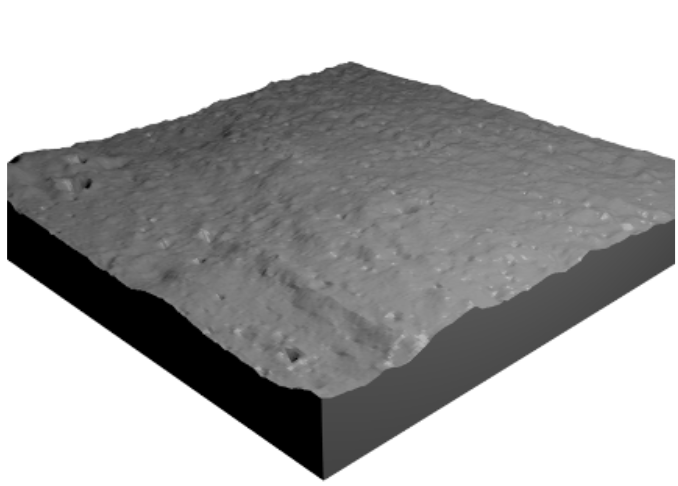
\includegraphics[keepaspectratio, scale=0.15]{images/NASA_moon.png}
    \subcaption{月面の例1}\label{fig:NASA_moon}
  \end{minipage}
  \begin{minipage}[b]{0.48\linewidth}
    \centering
    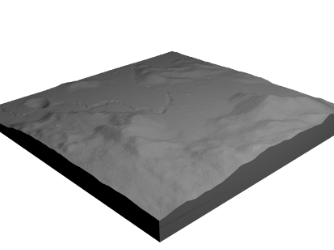
\includegraphics[keepaspectratio, scale=0.3]{images/NASA_moon2.png}
    \subcaption{月面の例2}\label{fig:NASA_moon2}
  \end{minipage}
  \caption{使用した月面の例}\label{fig:NASA_moons}
\end{figure}



\subsubsection{ボクセル化について}
本研究では,三次元分布の可視化をする際にその特徴をボクセルによって表現することとした.このボクセルの解像度によって地表面の起伏度合いを調整できることと,その起伏度合いが視覚的に伝わりやすいためである.ここでは月面データをボクセル化する方法について具体的に述べていく.まずはボクセルの解像度を設定する.ここでは仮にボクセルの解像度を256\times256\times64とする.地表のメッシュ三角形の頂点座標を取得し,256\times256の各格子内にある頂点の平均値をその代表点とする.[図\ref{fig:mesh_point}]それらの点の最大値が高さ方向の解像度の64マス目となる.このようにして0マス目からその格子の点の高さまでを点で埋めることで,0と1で表現された256\times256\times64の座標データが出来上がる.これに従って$1\mathrm{\,m}$\times$1\mathrm{\,m}$\times$1\mathrm{\,m}$の矩形を描くことでボクセルを表現する.

\begin{figure}[b]
  \centering
  \begin{minipage}[b]{0.37\linewidth}
    \centering
    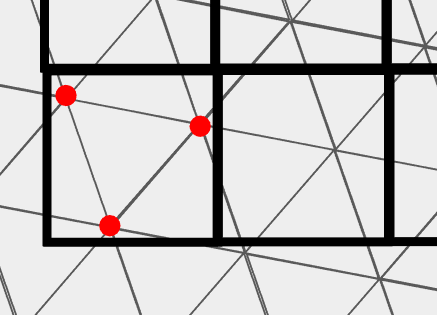
\includegraphics[keepaspectratio, scale=0.2]{images/mesh1.png}
    \subcaption{メッシュ三角形の頂点座標}\label{fig:mesh1}
  \end{minipage}
  \begin{minipage}[b]{0.35\linewidth}
    \centering
    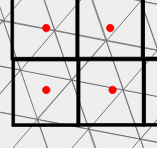
\includegraphics[keepaspectratio, scale=0.45]{images/mesh2.png}
    \subcaption{頂点の平均値による代表点}\label{fig:mesh2}
  \end{minipage}
  \caption{使用した月面の例}\label{fig:mesh_point}
\end{figure}


\subsubsection{GANを用いた地形データ生成について}
三次元ボクセルの高さ方向の分散により,不整地の起伏度合いを表現した.使用したGANモデルの構造を以下の図\ref{fig:3d_gan}に示す.データの入力方法は,正規分布に従った乱数の平均と標準偏差の値を入力する方法,画像をエンコードした後の平均と標準偏差の値を入力する方法,深度カメラ等を用いて取得した画像から作成した三次元のボクセル座標をエンコードした後,その平均と標準偏差の値を入力する方法の3種類となっている.月面データを32\times32\times32に分割したボクセルにし,その三次元座標をGANの入力として学習を行った出力結果が図\ref{fig:voxel}である.

\begin{figure}[b]
  \begin{center}
   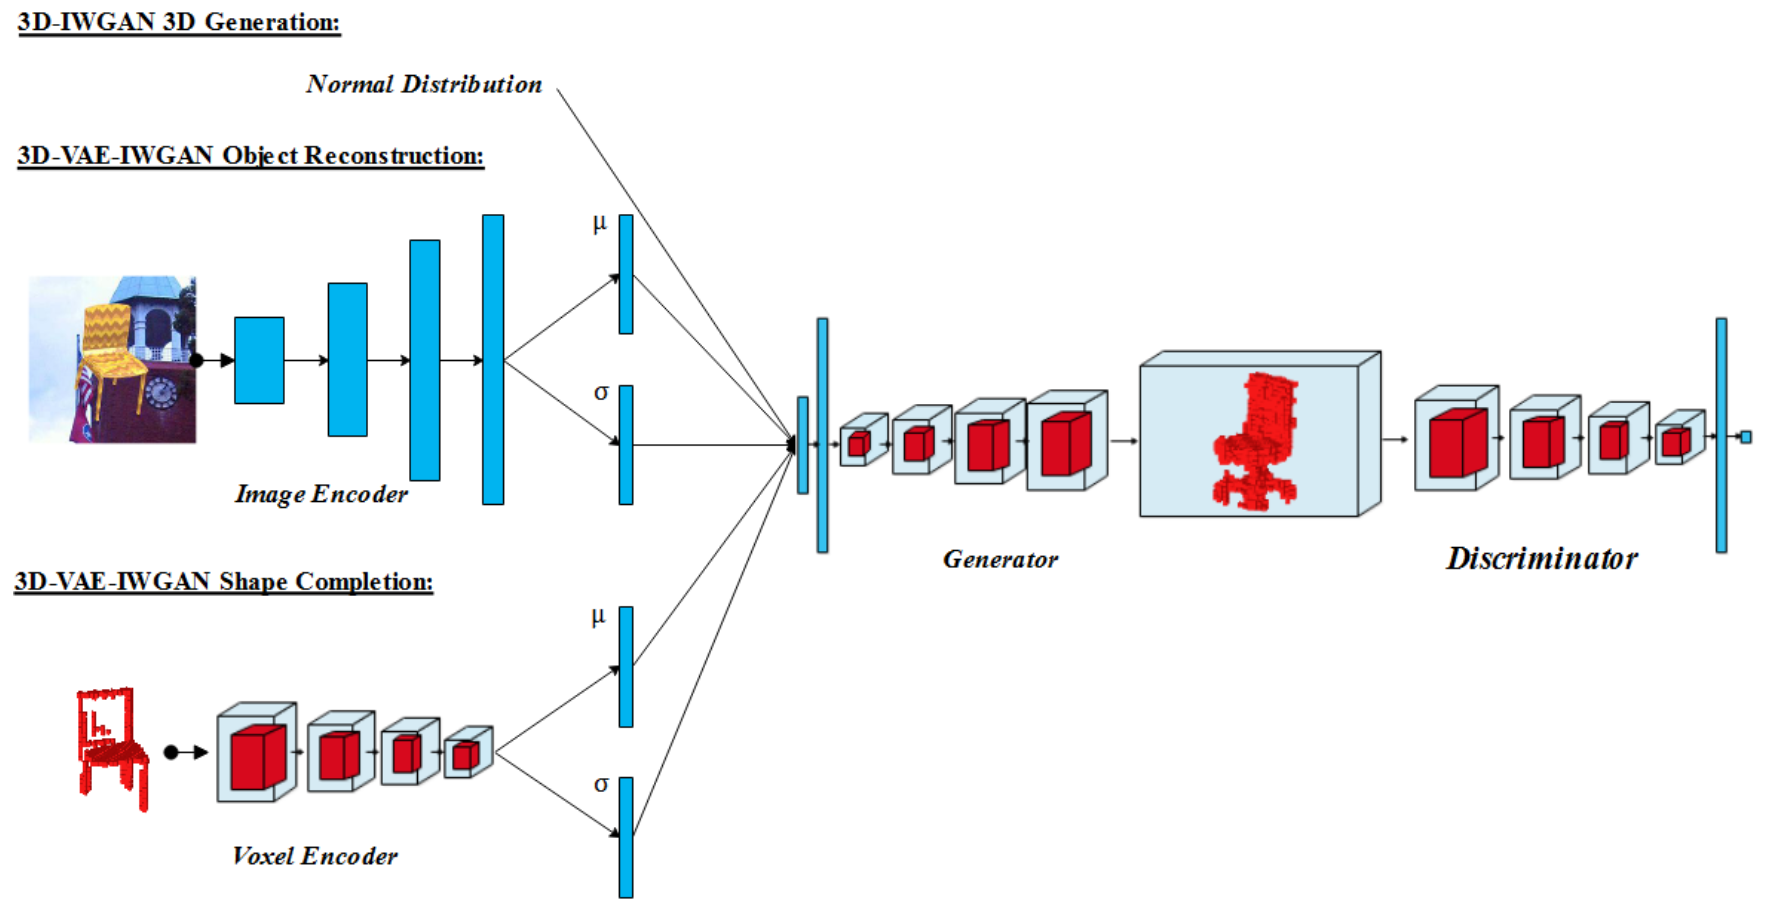
\includegraphics[width=1.0\linewidth]{images/3d_gan.png}
   \caption{3D-IWGANのモデル構造}
   \label{fig:3d_gan}
  \end{center}
\end{figure}

\begin{figure}[b]
  \begin{center}
   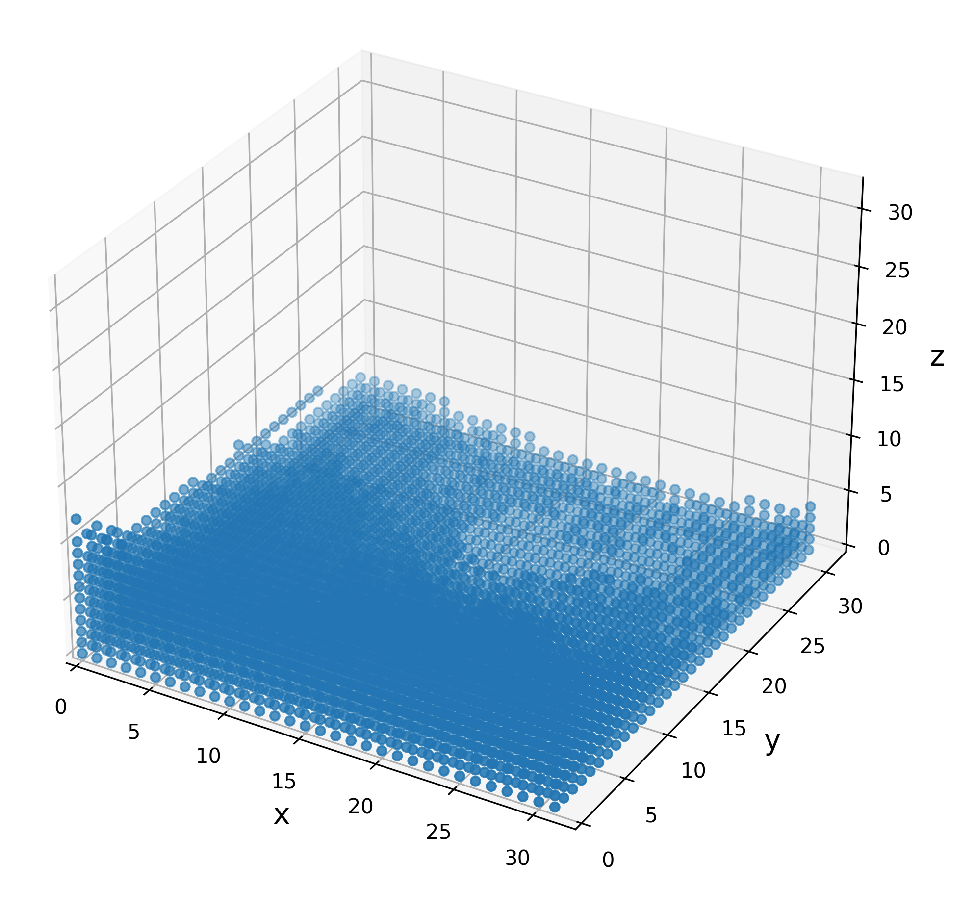
\includegraphics[width=0.6\linewidth]{images/voxel.png}
   \caption{GANでの学習結果}
   \label{fig:voxel}
  \end{center}
\end{figure}


\subsubsection{メッシュ化について}
ボクセル化した地形を元の月面のようになだらかな地表に変換するため,本研究ではボクセルの点からスプライン補間\cite{bunken3}によって求めた曲線に基づいてメッシュデータに変換する方法を用いた.スプライン補間はある複数の点を全て通る曲線の多項式を求める方法である.仮にxy平面の三次のスプライン補間を行う場合,以下のような多項式になる.ここでSは曲線が通る各点のy座標,nは曲線が通る点の数,そして最終的に求めるのは各項の係数となる.\\
\begin{math}
    S_0(x)  = a_0 + b_0(x - x_0) + c_0(x - x_0)^{2} + d_0(x - x_0)^{3}\\
    S_1(x)  = a_1 + b_1(x - x_1) + c_1(x - x_1)^{2} + d_1(x - x_1)^{3}\\
    S_2(x)  = a_2 + b_2(x - x_2) + c_2(x - x_2)^{2} + d_2(x - x_2)^{3}\\
    \vdots\\
    S_j(x)  = a_j + b_j(x - x_j) + c_j(x - x_j)^{2} + d_j(x - x_j)^{3}\\
    \vdots\\
    S_{n-1}(x)  = a_{n-1} + b_{n-1}(x - x_{n-1}) + c_{n-1}(x - x_{n-1})^{2} + d_{n-1}(x - x_{n-1})^{3}\\
\end{math}
生成した地形では次数を10と設定したため,多項式は以下のようになり,求める係数は
\begin{math}a \sim k\end{math}
となる.\\
\begin{math}
    S_{n-1}(x)  = a_{n-1} + b_{n-1}(x - x_{n-1}) + c_{n-1}(x - x_{n-1})^{2} + d_{n-1}(x - x_{n-1})^{3}\ldots + k_{n-1}(x - x_{n-1})^{10}
\end{math}

これにはPythonの数値解析ライブラリであるSciPyからscipy.interpolate.bisplrepという関数を呼び出すことで自動で計算を行った.
この曲線にそって三角形メッシュの頂点を決定してメッシュ化を行う.以下の図\ref{fig:mesh_moons}は生成した月面のボクセルデータとそれを元にメッシュ化した月面データの例である.高さの離れた点が隣接していると,スプライン曲線の特性上例の4のように極端に鋭利な地形領域ができてしまう場合があった.

\begin{figure}[b]
  \centering
  \begin{minipage}[b]{0.49\linewidth}
    \centering
    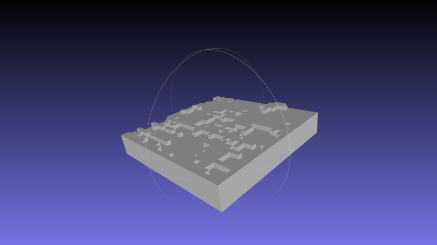
\includegraphics[keepaspectratio, scale=0.25]{images/voxel1.png}
    \subcaption{ボクセル化した月面の例1}\label{fig:voxel1}
  \end{minipage}
  \begin{minipage}[b]{0.49\linewidth}
    \centering
    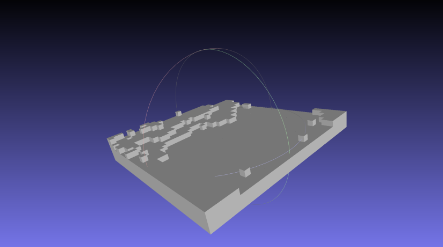
\includegraphics[keepaspectratio, scale=0.25]{images/voxel2.png}
    \subcaption{ボクセル化した月面の例2}\label{fig:voxel2}
  \end{minipage}
  \caption{ボクセル化した月面の例}\label{fig:voxel_moons}
\end{figure}

\begin{figure}[b]
  \centering
  \begin{minipage}[b]{0.49\linewidth}
    \centering
    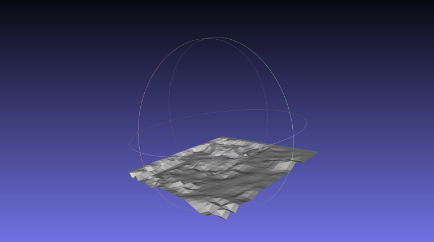
\includegraphics[keepaspectratio, scale=0.25]{images/spline1.png}
    \subcaption{メッシュ化した月面の例1}\label{fig:spline1}
  \end{minipage}
  \begin{minipage}[b]{0.49\linewidth}
    \centering
    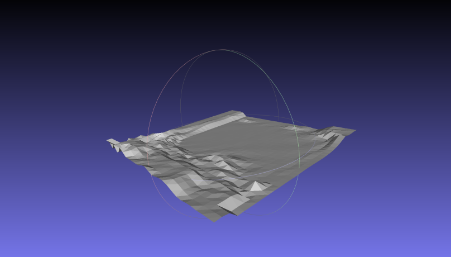
\includegraphics[keepaspectratio, scale=0.24]{images/spline2.png}
    \subcaption{メッシュ化した月面の例2}\label{fig:spline2}
  \end{minipage}
  \caption{スプライン近似によってメッシュ化した月面の例}\label{fig:mesh_moons}
\end{figure}

\subsection{ロボットの構成}
使用するロボットには,外界のセンシング機能と不整地に対する一定の走破性能を持ったハードウェアがそれぞれ要求される.そこで使用するロボットには,図\ref{fig:fig}のような径の大きな2つのタイヤと2つのキャスタ,深度カメラを4方向に搭載した.
このロボットは,ROS及びGazeboシミュレーターの管理団体であるOpen RoboticsとロボットメーカーROBOTIS(ロボティズ)が共同開発したTurtlebot3\cite{bunken4}のWaffleモデルをもとにしており,各寸法は図\ref{fig:turtlebot}のようになっている.タイヤ径はこの3.5倍に設定しており,4方向の深度カメラは水平方向に対し45度下に傾けた状態にしている.深度カメラの画像サイズは320\times320とした.

\begin{figure}[t]
  \begin{center}
   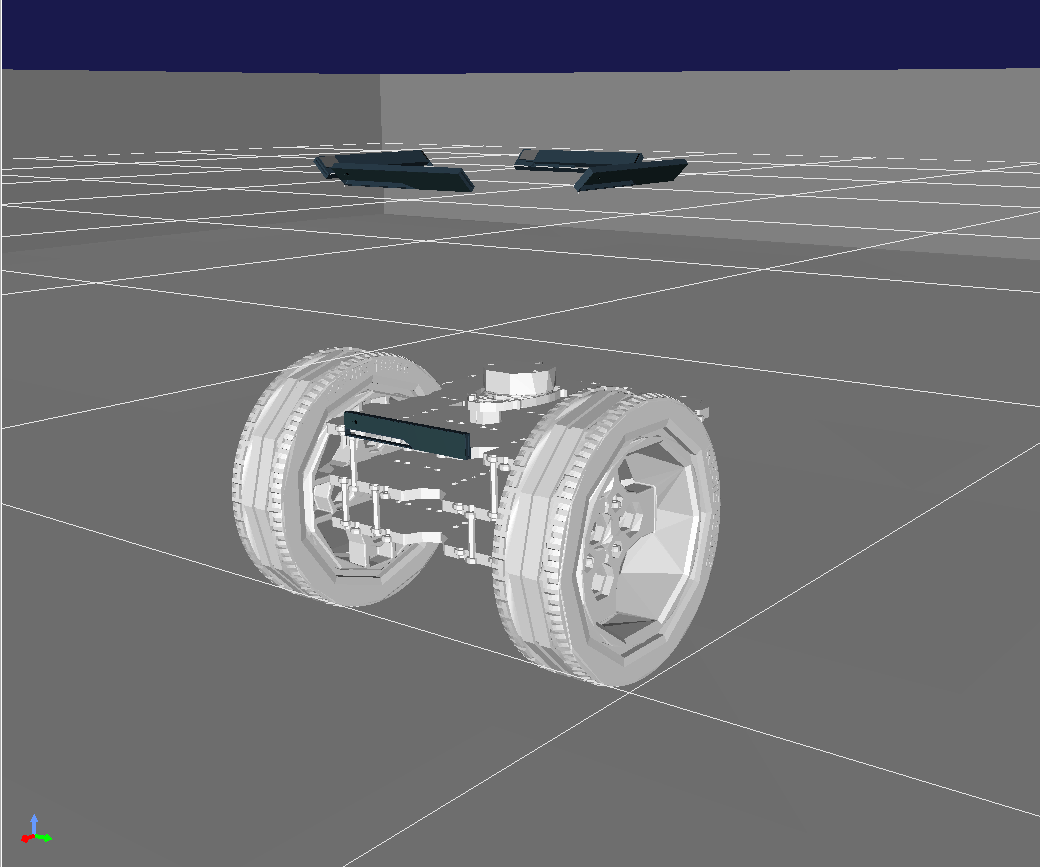
\includegraphics[width=0.4\linewidth]{images/robot_visual.png}
   \caption{ロボットの構成}
   \label{fig:fig}
  \end{center}
 \end{figure}


\begin{figure}[t]
  \begin{center}
   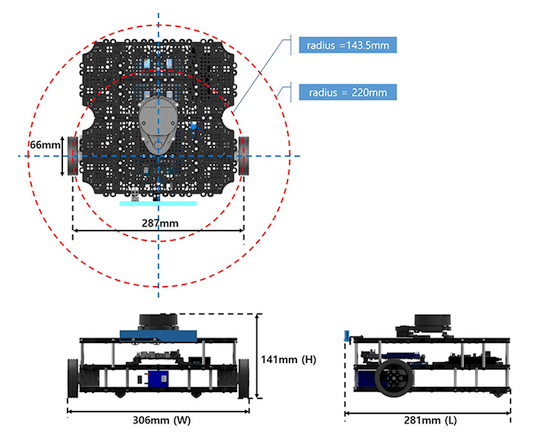
\includegraphics[width=0.7\linewidth]{images/turtlebot.png}
   \caption{TurtleBot3 Waffle}
   \label{fig:turtlebot}
  \end{center}
 \end{figure}


\subsection{走行計画手法}
走行計画として,4つの深度カメラから得られた画像から走行可能な方位を選択する方法を用いた.事前に生成した地形を用いて走行実験を行い,ある方位に走行可能だった場合はsafe(図\ref{fig:labeling}左) として 0,転倒や脱輪により探査続行不可になった場合はその直前の画像に danger(図\ref{fig:labeling}右)として 1 をラベリングする.そのデータに対し出力が 0 から 1 になるよう機械学習し,走行中に推論した結果最も 0 に近い値を出力した方位に向かうようにした.例えば図\ref{fig:planning}のような場合には,ロボットは前方向に進む.

\begin{figure}[t]
  \centering
  \begin{minipage}[b]{0.47\linewidth}
    \centering
    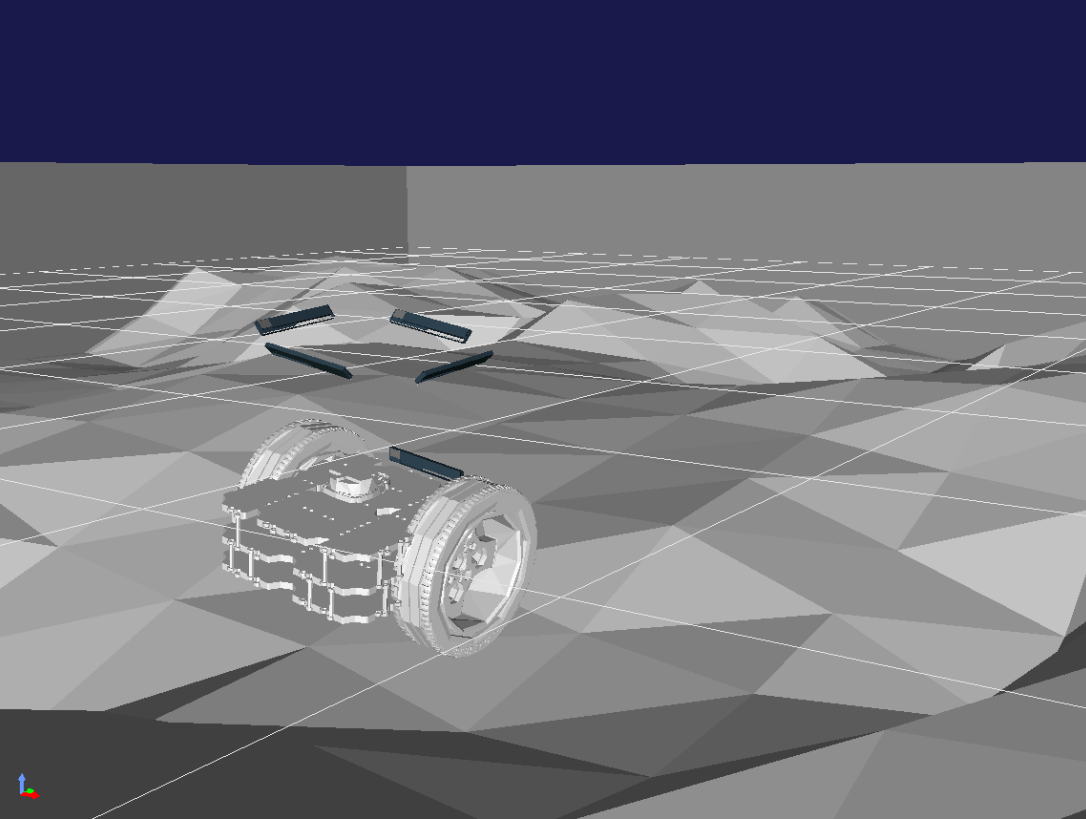
\includegraphics[keepaspectratio, scale=0.1]{images/safe.png}
    \subcaption{safeの時}\label{fig:safe}
  \end{minipage}
  \begin{minipage}[b]{0.47\linewidth}
    \centering
    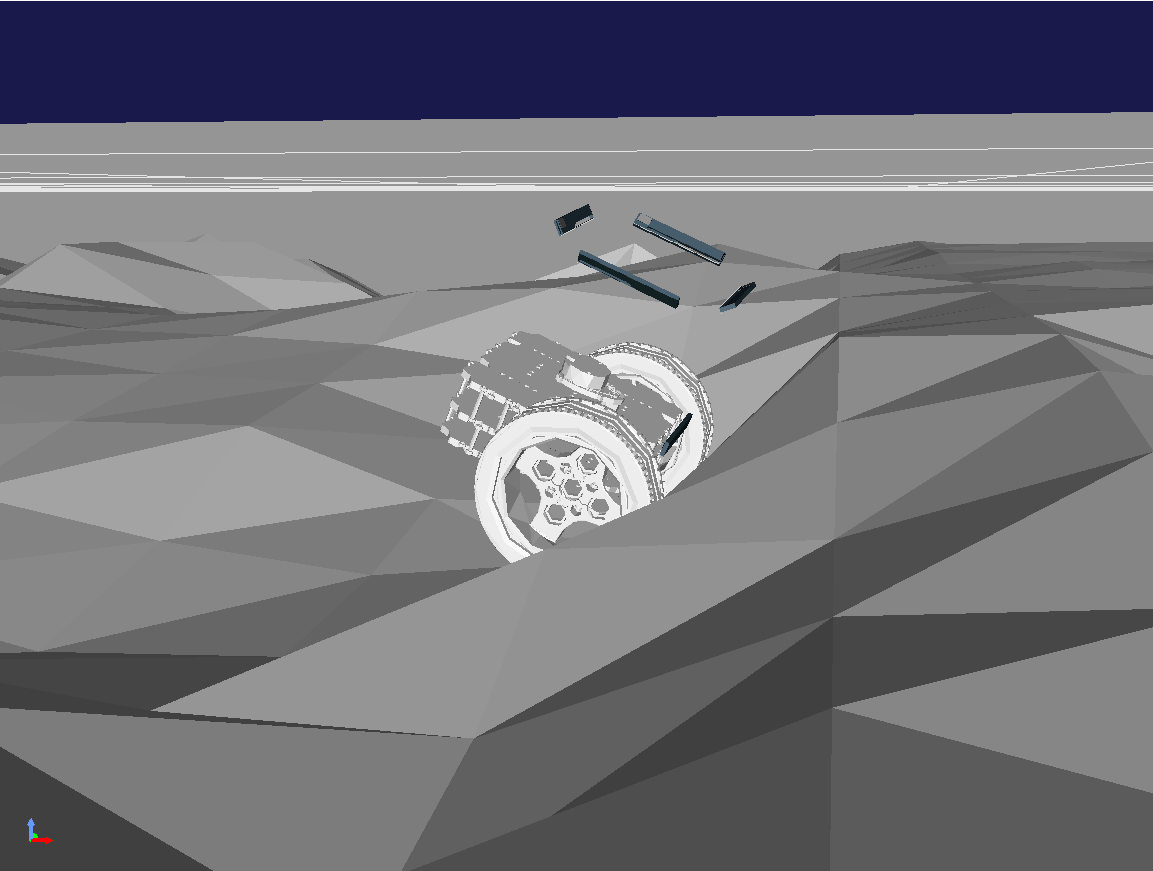
\includegraphics[keepaspectratio, scale=0.096]{images/stack.png}
    \subcaption{dangerの時}\label{fig:stack}
  \end{minipage}
  \caption{ラベリングのイメージ}\label{fig:labeling}
\end{figure}

\begin{figure}[t]
  \begin{center}
    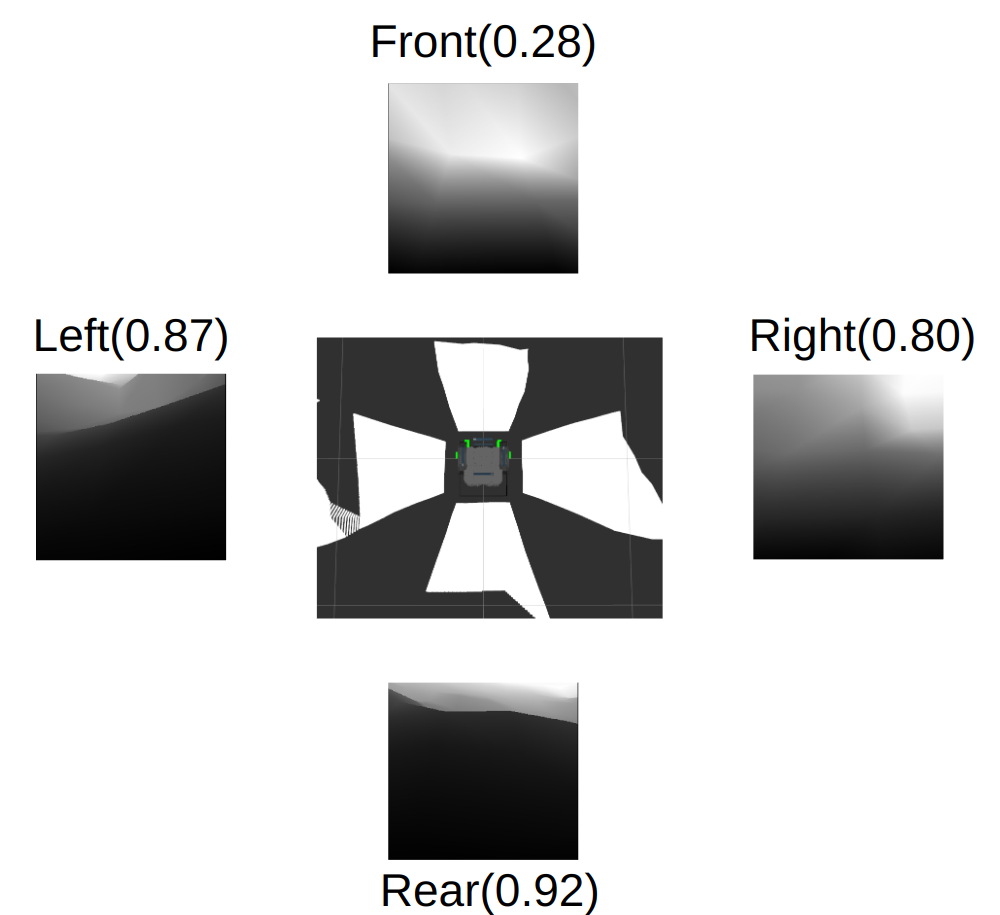
\includegraphics[width=0.6\linewidth]{images/planning.png}
    \caption{4方向からの深度画像と推論イメージ}
    \label{fig:planning}
  \end{center}
\end{figure}

\subsection{実験方法}
予め生成した複数の不整地上を手動操作でロボットに走行させ,機械学習用データを収集する。画像数は計10000枚ほどであり,それぞれにsafeとdangerをラベリングした.学習モデルにはCNN(Convolutional Neural Network) を使用した.上記のデータを用いて学習を行い,再度生成した不整地上をロボットに走行させながらその軌跡を保存する.走行するマップ範囲内での軌跡の含有率をロボットの走破性と定義した.\cite{bunken2}シミュレーションにはロボット用統合 GUI ソフトウェアであるchoreonoid を用いた.このシミュレーション環境上に月面と$6 \mathrm{\,m}$\times$6\mathrm{\,m}$の壁を周囲に配置し,それをマップの範囲とした.[図\ref{fig:choreonoid}]

% \begin{figure}[b]
%   \begin{center}
%    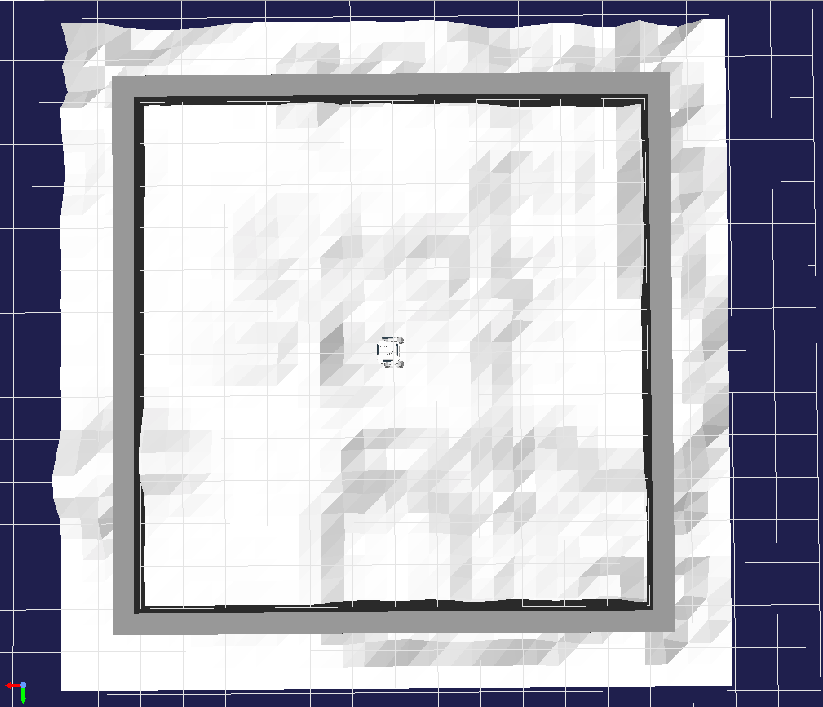
\includegraphics[width=0.5\linewidth]{images/choreonoid.png}
%    \caption{実験用マップ}
%    \label{fig:choreonoid}
%   \end{center}
%  \end{figure}

\subsection{生成地形の評価}
本研究では以下の2つの点からロボットを走行させることで地形データの評価をすることとした.
\begin{enumerate}
  \item 分散や標準偏差といった統計量が極端に離れている地形を生成した場合,特徴量の範囲が広い汎用的な地形データを収集できるが,学習用データとして用いて走行させた際に実際の地形に対する走破性向上に繋がるかは未知数となる.
  \item 仮に統計的に近い地形データを生成できたとしても,ロボットの座標や地表面のある隣接した領域どうしの関係性によって走破性は左右する.
\end{enumerate}
学習済みモデルを用いて,生成した不整地上と元の月面上をそれぞれ2分間走行させた際の軌跡に対し,マップの走破性を比較することで生成地形の有用性を評価した.使用した元の月面と生成した月面,走行した結果はそれぞれ下図のようになった.ここで,各グラフの中心がロボットの開始位置で,軌跡の止まった点がロボットの走行終了地点である.生成した地形の高さ方向の分散が起伏度合いに影響を与えるため,生成した月面2のような分散の小さいものを用いると極端に走破性が上がってしまった.逆に起伏が過度に激しいと,走破性が極端に下がり,かつロボットを配置したスタート地点に依存した走破性になってしまう.

\begin{figure}[t]
  \centering
  \begin{minipage}[b]{0.49\linewidth}
    \centering
    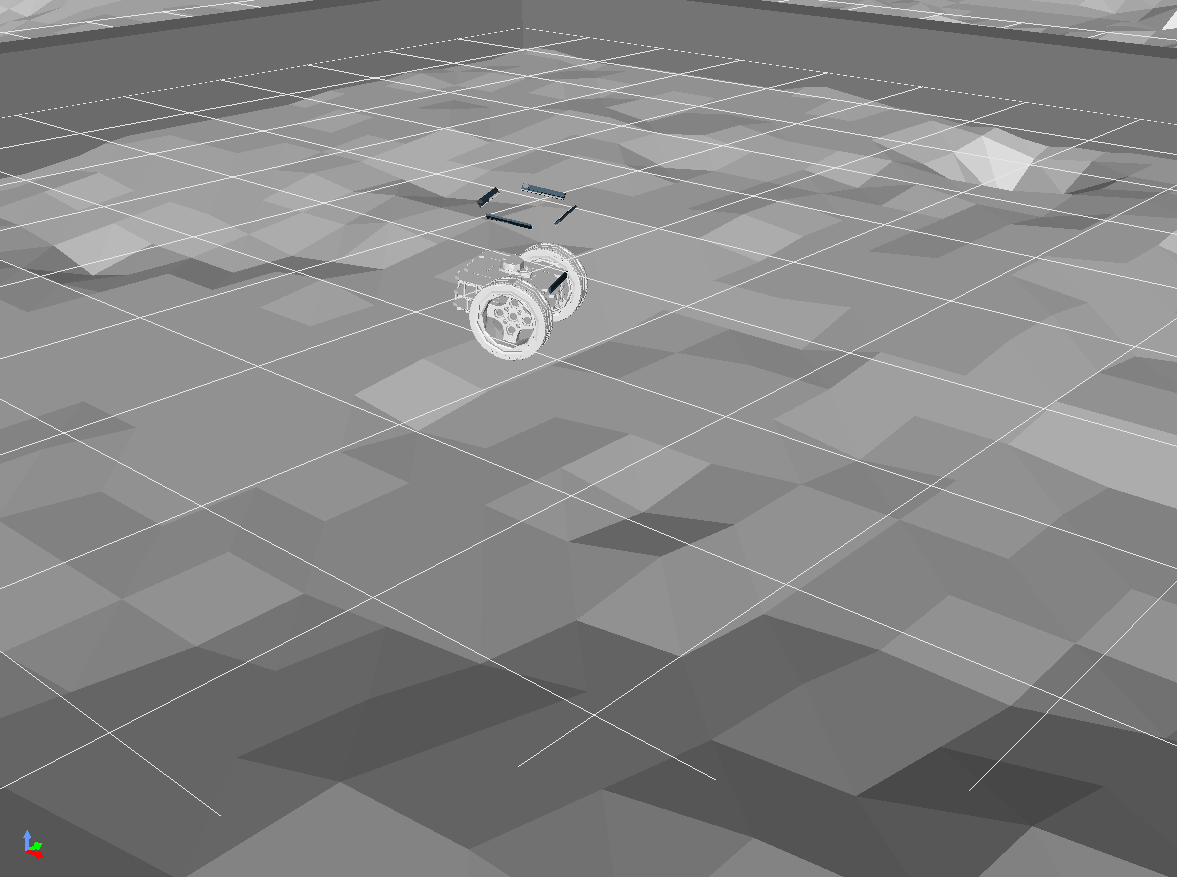
\includegraphics[keepaspectratio, scale=0.096]{images/origin_moon_field3.png}
    \subcaption{元の月面1}\label{fig:origin_moon_field3}
  \end{minipage}
  \begin{minipage}[b]{0.49\linewidth}
    \centering
    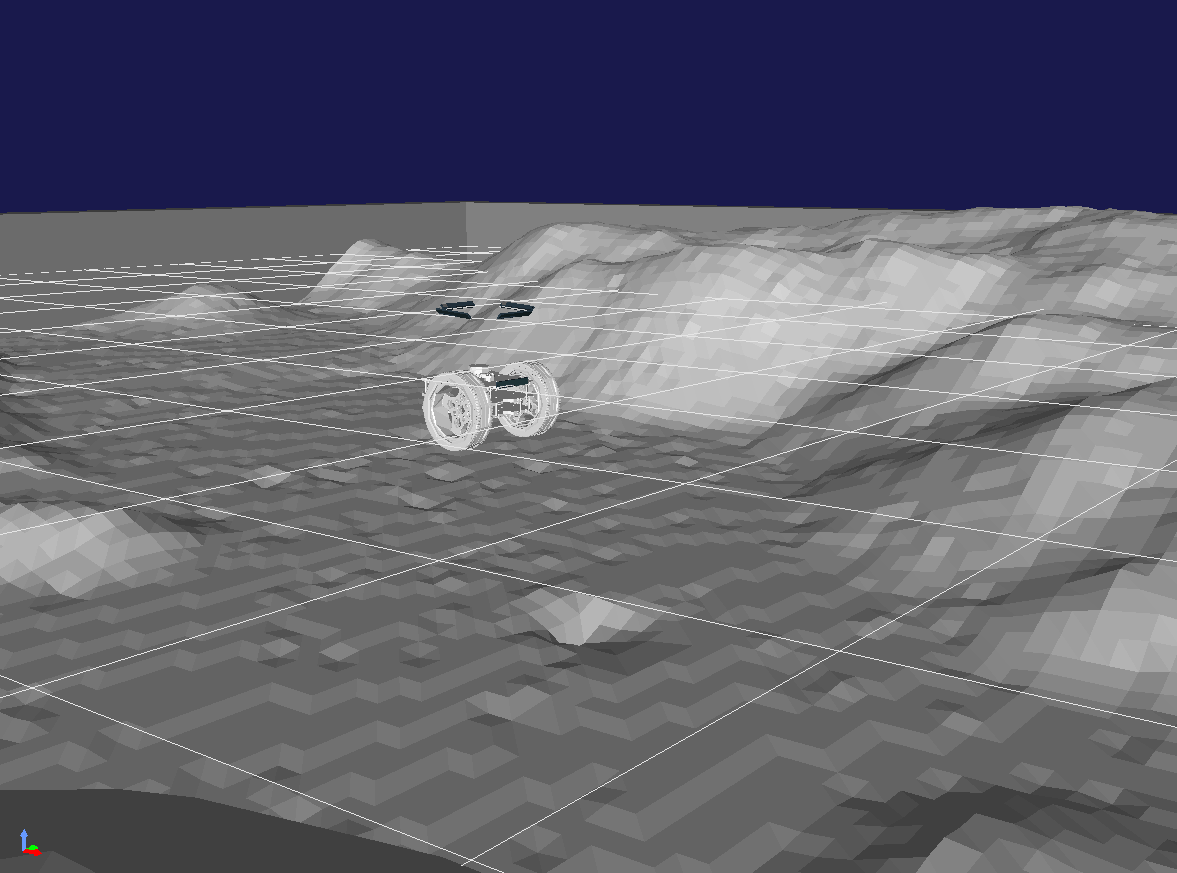
\includegraphics[keepaspectratio, scale=0.096]{images/original_moon_field4.png}
    \subcaption{元の月面2}\label{fig:original_moon_field4}
  \end{minipage}
  \caption{元の月面}
\end{figure}

\begin{figure}[t]
  \centering
  \begin{minipage}[b]{0.49\linewidth}
    \centering
    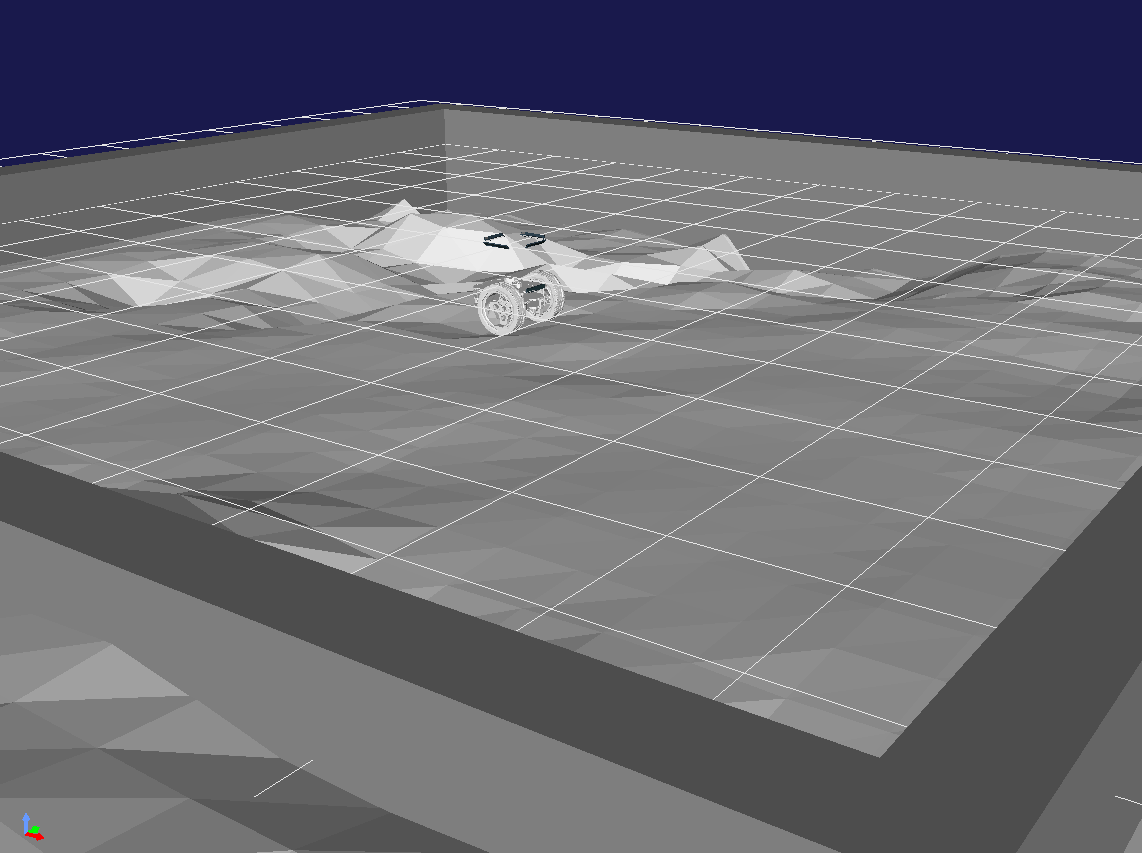
\includegraphics[keepaspectratio, scale=0.096]{images/generate_field3.png}
    \subcaption{生成した月面1}\label{fig:generate_field3}
  \end{minipage}
  \begin{minipage}[b]{0.49\linewidth}
    \centering
    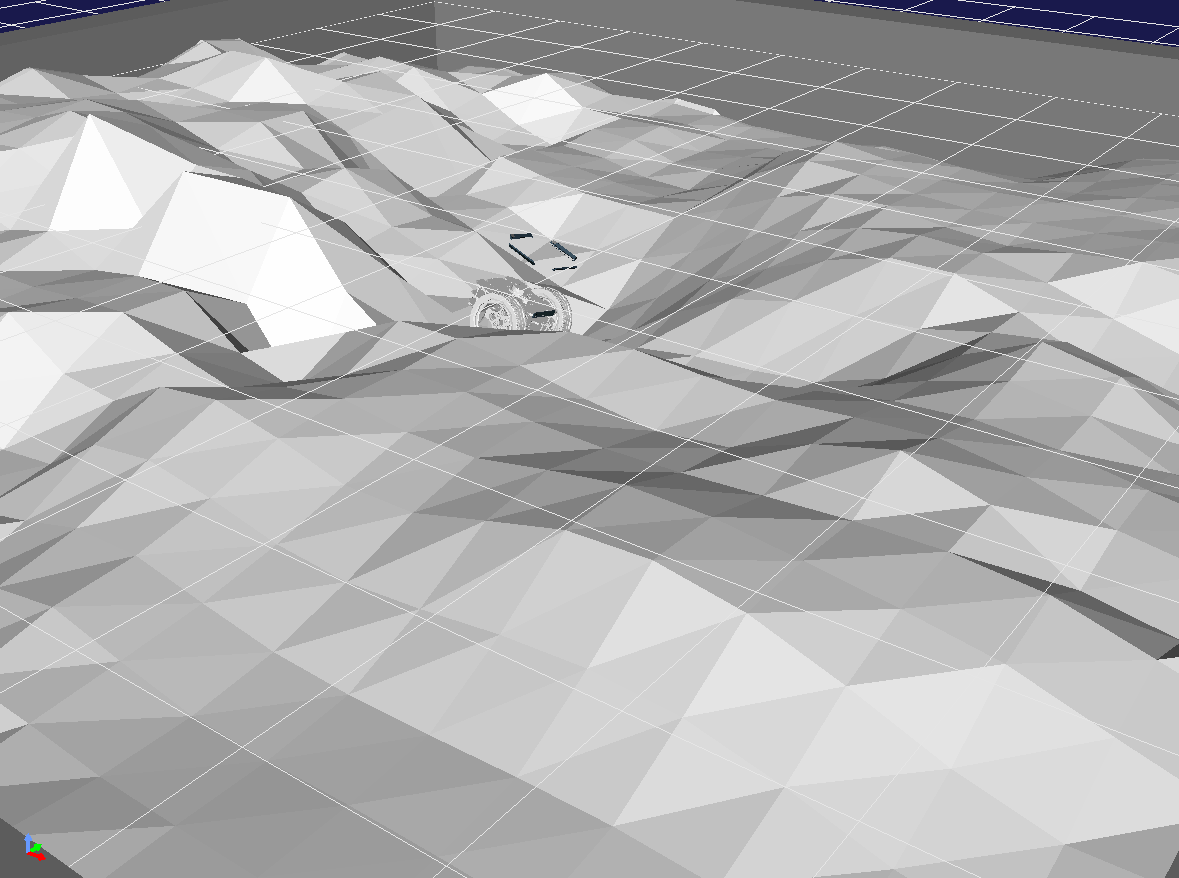
\includegraphics[keepaspectratio, scale=0.096]{images/generate_field4.png}
    \subcaption{生成した月面2}\label{fig:generate_field4}
  \end{minipage}
  \caption{生成した月面}
\end{figure}

\begin{figure}[t]
  \centering
  \begin{minipage}[b]{0.47\linewidth}
    \centering
    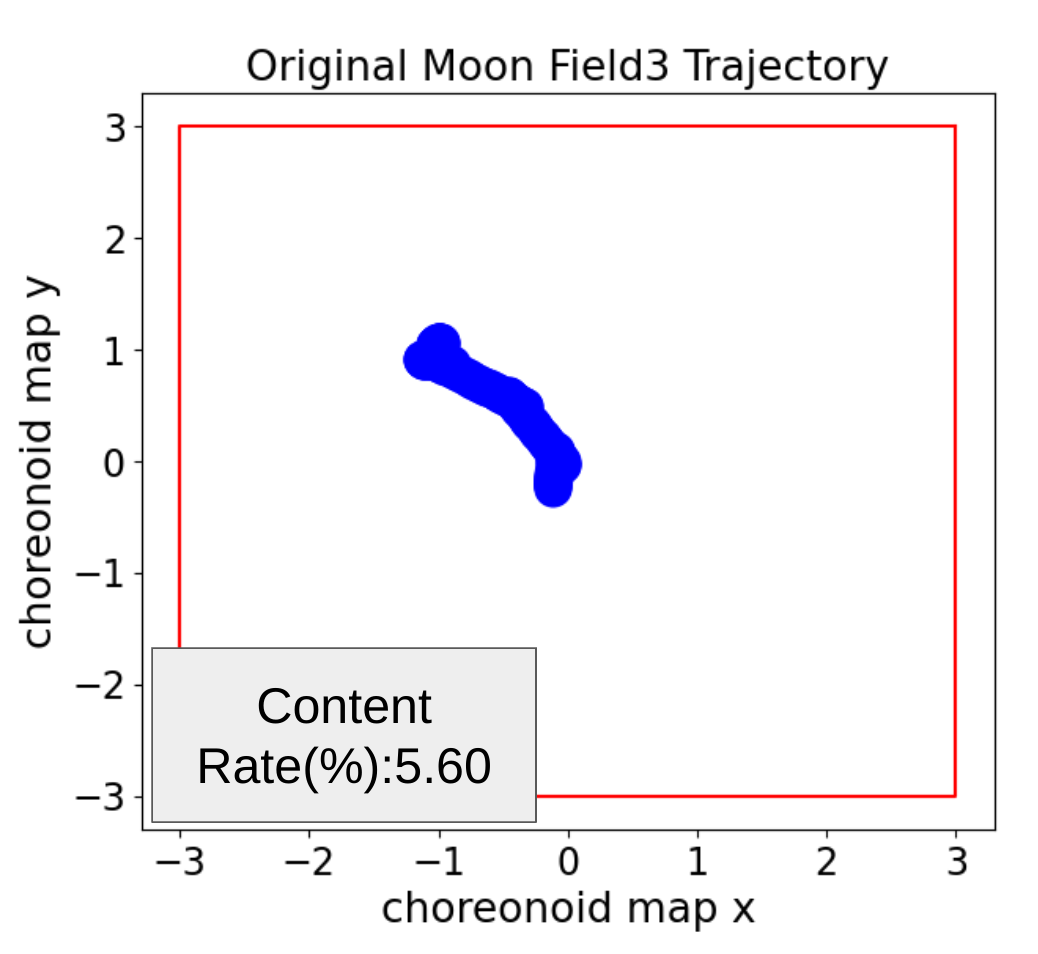
\includegraphics[keepaspectratio, scale=0.096]{images/origin_moon_trajectory3.png}
    \subcaption{元の月面1}\label{fig:origin_moon_trajectory3}
  \end{minipage}
  \begin{minipage}[b]{0.47\linewidth}
    \centering
    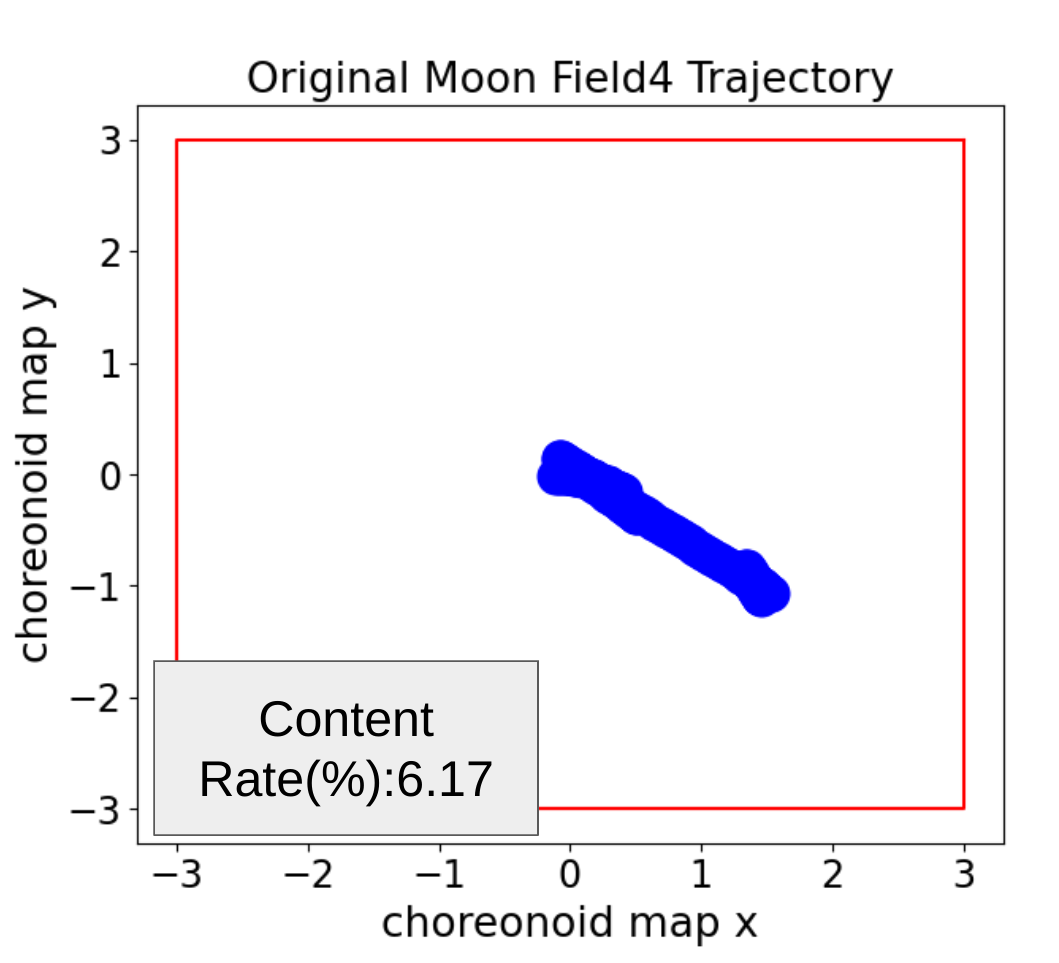
\includegraphics[keepaspectratio, scale=0.096]{images/origin_moon_trajectory4.png}
    \subcaption{元の月面2}\label{fig:origin_moon_trajectory4}
  \end{minipage}
  \caption{元の月面}
\end{figure}

\begin{figure}[t]
  \centering
  \begin{minipage}[b]{0.47\linewidth}
    \centering
    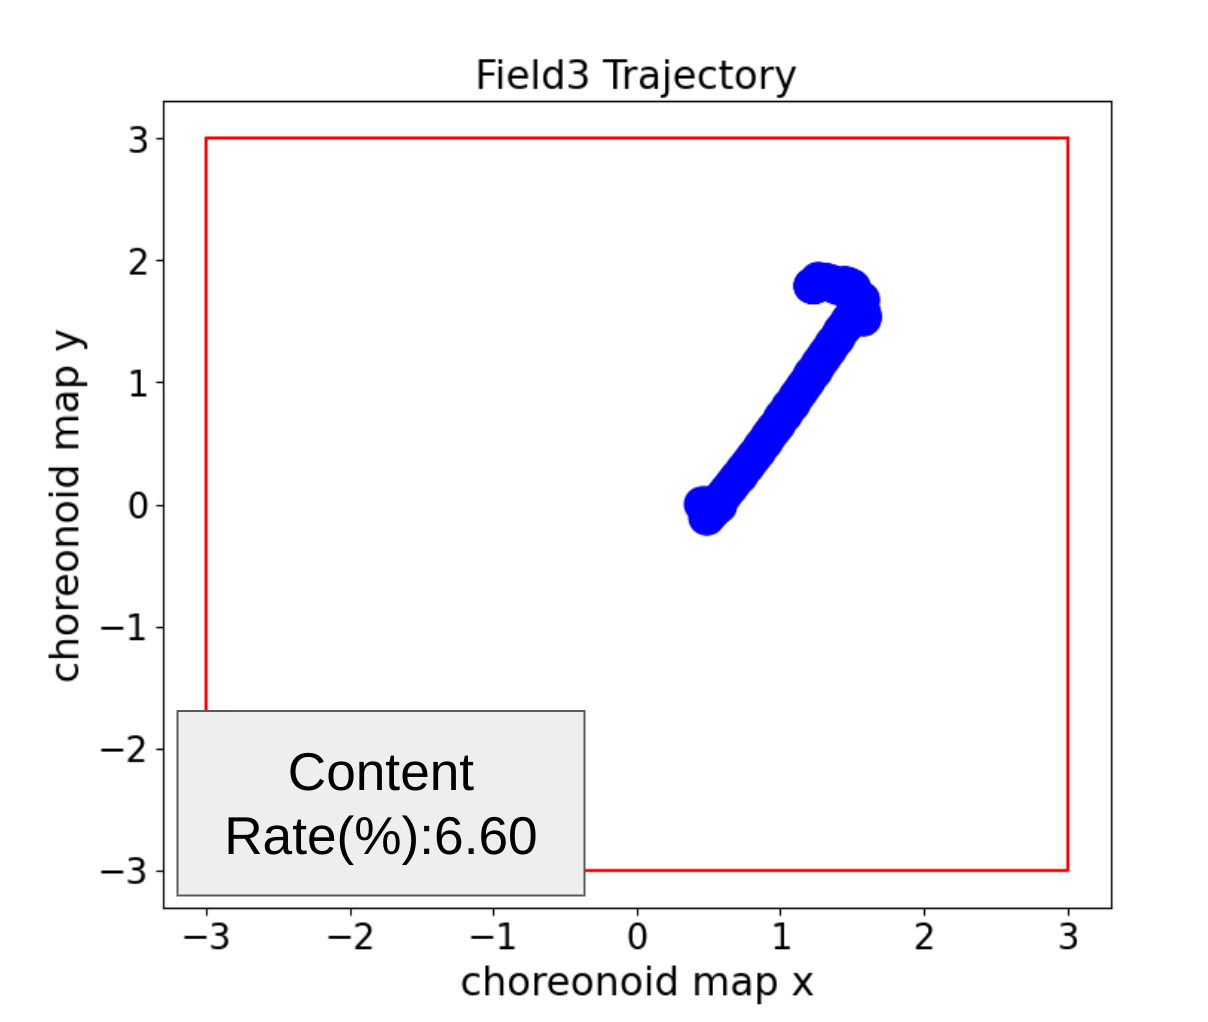
\includegraphics[keepaspectratio, scale=0.096]{images/generate_trajectory3.png}
    \subcaption{生成した月面1}\label{fig:generate_trajectory3}
  \end{minipage}
  \begin{minipage}[b]{0.47\linewidth}
    \centering
    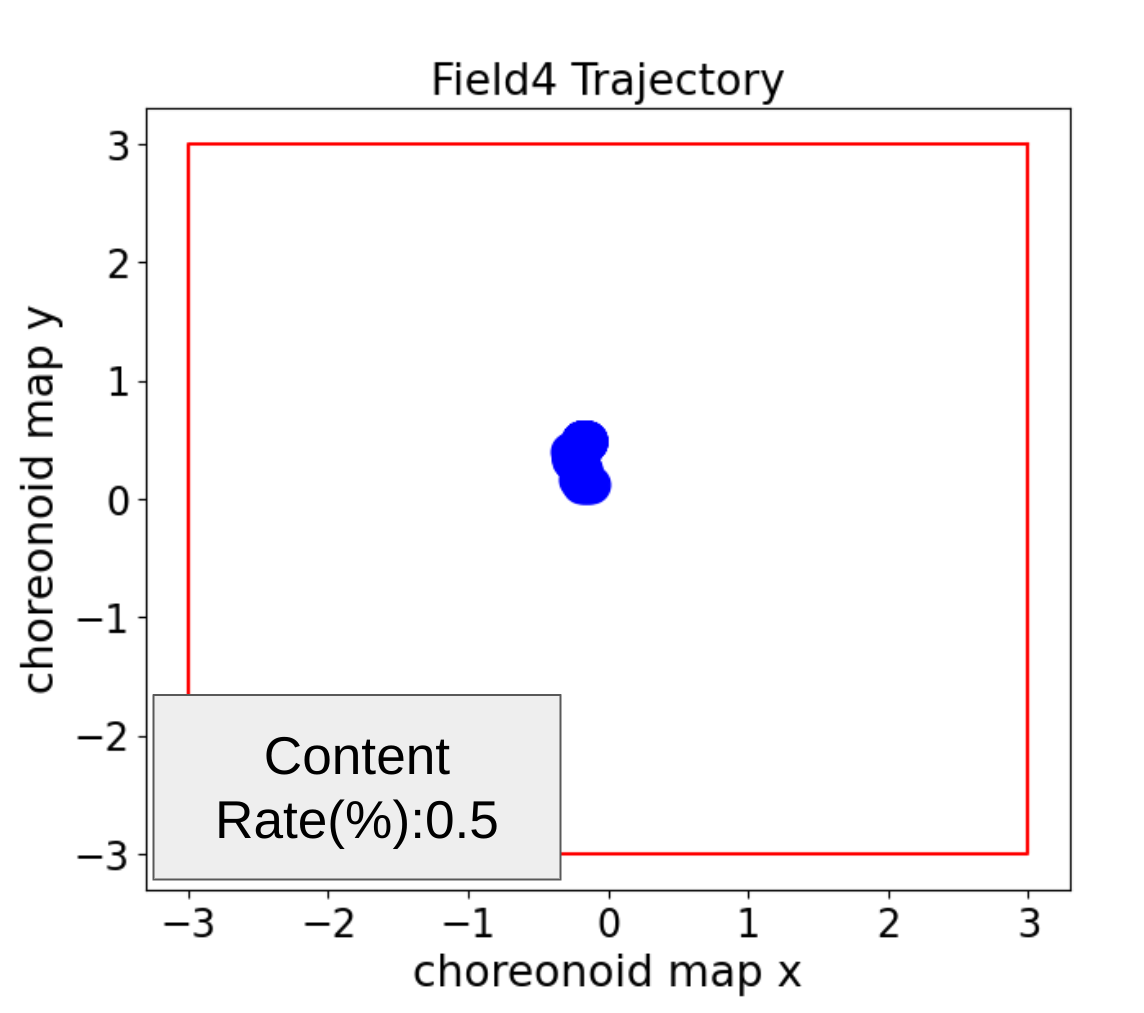
\includegraphics[keepaspectratio, scale=0.096]{images/generate_trajectory4.png}
    \subcaption{生成した月面2}\label{fig:generate_trajectory4}
  \end{minipage}
  \caption{生成した月面}
\end{figure}


\section{おわりに}

\subsection{まとめ}
本研究では3D-IWGANを用いて不整地を生成することで,走行計画に必要な学習用データを効率的かつ大規模に用意し,その走破性評価による実験フレームワークの作成を行った.3章で述べたとおり,生成した地形が走行計画の学習用データとしての有用性があるかは,統計的な特徴量だけで判断するのは難しく,実際にロボットを走行させて評価する必要があることが分かった.ここでは,マップ内をロボットに走行させた軌跡の含有率が近いデータが元の地形データと類似していると判断し,更にその有用性を評価できた.また,本研究での実験フレームワークによって元の月面データの走破結果に近い生成地形を用いることで,少数の地形データで走行計画に必要な機械学習用データを効率的に収集できることが分かった.


\subsection{今後の課題}
シミュレーション環境の実験フレームワークだけでなく,現実環境で実機を用いた検証を行えるような方法を検討する.また,本研究では月面を未知環境の例として取り扱ったが,災害現場等についても同様な実験が行えるか検討する.

% %図の入れ方
% \begin{figure}[tb]
%   \centering
%   \large
%   \begin{tikzpicture}
%     \draw rectangle++(4.5,3);
%     \clip rectangle++(4.5,3);
%     \foreach\x in{0,1,2,3,4}{
%       \foreach\y in{0,1,2,3,4,5,6}{
%         \path(\x*1.5-\y*0.5,\y*0.6)node[rotate=10,text=gray]{\sffamily\bfseries\itshape Sample };
%       }
%     }
%   \end{tikzpicture}
%   % eps 画像を貼る場合は includegraphics をお使いください。
%   % \includegraphics[width=45mm]{samplefig2.eps}
%   \caption{サンプル画像}
%   \label{fig:sample}
% \end{figure}



%% 謝辞(必要な場合のみ)
%%\begin{acknowledgements}
%%\end{acknowledgements}

%% 謝辞(必要な場合のみ)
%\begin{acknowledgements}
%    Thanks.
%\end{acknowledgements}

\small
\begin{thebibliography}{9}
%%%%%%%%%%%%%%%%%%%%%%%%%%%%%%%%%%%%%%%%%%%%%%%%%%%%%%%%%%%%%%%%%%%%%%%%%%%%%%%

\bibitem{bunken1}
``Jaxa 解決すべき技術課題'',
  \url{https://www.ihub-tansa.jaxa.jp/introduction/themes.html}
\bibitem{bunken2}
西村祐輝:
  ``強化学習を用いた自律多脚車輪型ロボットの脱出行動の環境適応. 2016.'',
\bibitem{bunken3}
David Meger Edward J. Smith:
  ``Improved adversarial systems for 3d object generation and
  reconstruction. 2017.'',
\bibitem{bunken4}
  ``スプライン補間について',
  \url{https://qiita.com/khidaka/items/84610cd890ecb8443d96}
\bibitem{bunken5}
  ``Turtlebot について',
  \url{https://www.besttechnology.co.jp/modules/onlineshop/index.php?fct=photop=191}
\bibitem{bunken6}
  高橋 友一清水 優:
  ``モデル化した不整地による評価フィールドを用いたレスキューロボットの動
  作・地図作成能力評価手法の提案. 2014.',
%%%%%%%%%%%%%%%%%%%%%%%%%%%%%%%%%%%%%%%%%%%%%%%%%%%%%%%%%%%%%%%%%%%%%%%%%%%%%%%
\end{thebibliography}

\end{document}
